\documentclass{standalone}

\usepackage{tikz}
\usepackage{tikz-qtree}

\begin{document}

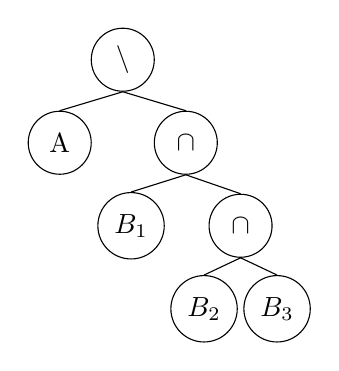
\begin{tikzpicture}

\tikzset{every tree node/.style={shape=circle, draw, minimum size=0.8cm}}
% \tikzset{level 1+/.style={sibling distance=0pt}}
% \tikzset{level 3/.style={sibling distance=12pt}}
\Tree [.{$\setminus$} [.A ] [.{$\cap$} [.{$B_1$} ] [.{$\cap$} [.{$B_2$} ] [.{$B_3$} ]  ] ] ]

\end{tikzpicture}

% \begin{tikzpicture}

% \tikzset{every tree node/.style={shape=circle, draw}}
% \Tree [.{$\cap$} [.{$B_1$} ] [.{$B_2$} ] ]

% \end{tikzpicture}

\end{document}